\placelogofalse
\begin{frame}{Vector Search: Graph Indexing}
\begin{columns}
\column{0.48\linewidth}
\centering
\begin{outline}
  \1 Proximity graph
  \2 Node for each vector
  \2 Edge for (approx) neighbors 
  \1 Query is a graph traversal 
\end{outline}

\column{0.48\linewidth}
\begin{outline}
  \1 For static data:
  \2 High recall!
  \2 Low latency!
  \1 For dynamic data:
  \2 Expensive to initialize
  \2 Expensive to update 
\end{outline}
\end{columns}

\begin{center}
\centering

% [trim={left bottom right top},clip]
\includegraphics[width=8.5cm, page=3, trim={0 9cm 14cm 0cm},clip]{assets/vec_db_figs.pdf}

\end{center}
\end{frame}
\placelogotrue
